% Full content of Vladimir_part/X5_slides/frames.tex, original frames 1-4.
% Only theme aliases, local 9 pt body, punctuation, subtitle placement and asset path adapted.
% model_scheme.jpg is a byte-identical copy of the explicitly requested original.
\begingroup
\setlength{\abovedisplayskip}{4pt}
\setlength{\belowdisplayskip}{4pt}
\setlength{\abovedisplayshortskip}{3pt}
\setlength{\belowdisplayshortskip}{3pt}
\setlength{\topsep}{2pt}
\setlength{\smallskipamount}{1pt}
\setbeamerfont{block title}{size=\VladimirText}
\setbeamerfont{block body}{size=\VladimirText}
% - 1. Схема исходного решения ------------------------
\begin{frame}[t]{Исходное решение: как устроен ансамбль}
  \VladimirText
  \noindent{Градиентный бустинг для прогноза РТО магазинов за март 2025 года}\par
  
  \begin{columns}[T,onlytextwidth]
    \begin{column}{0.42\textwidth}
      \begin{block}{Подготовка признаков}
        \VladimirText Около \hl{380 признаков}: лаги, скользящие средние, агрегаты и темпы прироста
      \end{block}
      
      \begin{block}{Отбор и настройка}
        \VladimirText Forward Selection: оценка важности на \hl{5 месячных фолдах} с периодическим пересчетом\par
        
        \VladimirText Optuna: взвешенная MAPE на \hl{3 фолдах}
      \end{block}
      
      \begin{block}{Итоговый прогноз}
        \VladimirText Четыре модели с разными признаками и двумя целевыми переменными. Далее - \hl{блендинг}
      \end{block}
    \end{column}
    \begin{column}{0.54\textwidth}
      \centering
      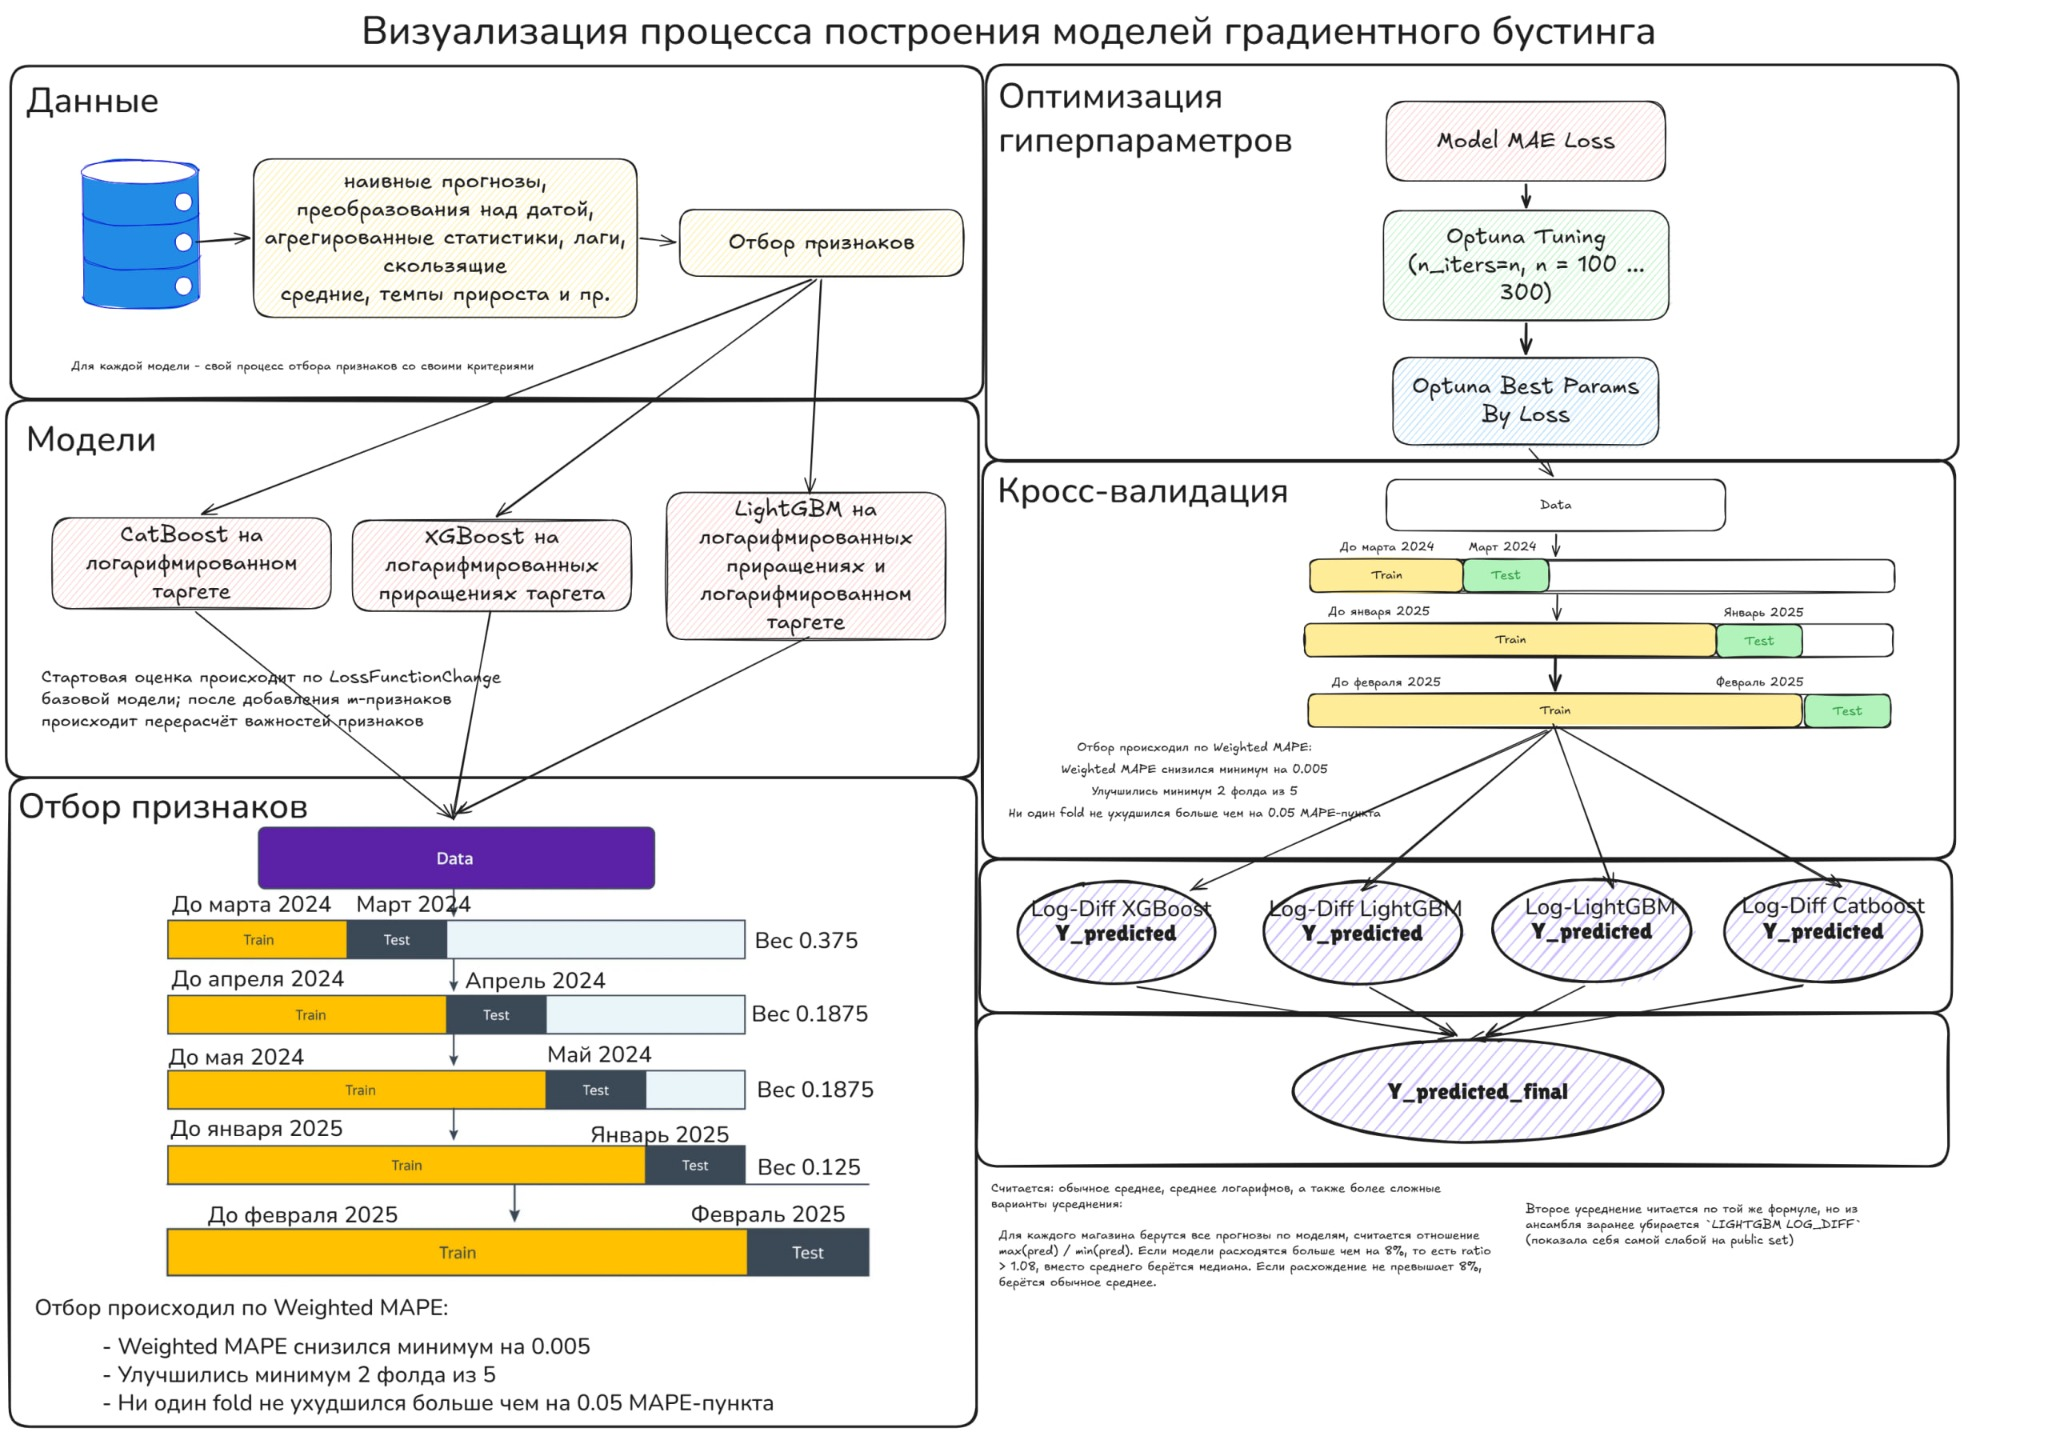
\includegraphics[width=\linewidth,height=.76\textheight,keepaspectratio]{assets/model_scheme.jpg}\par
      
      {\color{hsegray}\fontsize{8}{9}\selectfont Подробная схема обучения, проверки и объединения моделей}
    \end{column}
  \end{columns}
\end{frame}

% - 2. Модели, блендинг и математическая идея -----------------
\begin{frame}[t]{Почему ансамбль может улучшать прогноз?}
  \VladimirText
  \noindent{Разные целевые переменные, наборы признаков и ошибки моделей}\par
  
  \begin{columns}[T,onlytextwidth]
    \begin{column}{0.47\textwidth}
      \begin{block}{Четыре модели в исходном решении}
        \VladimirText
        \setlength{\tabcolsep}{4pt}
        \renewcommand{\arraystretch}{.95}
        \begin{tabular}{@{}ll@{}}
          \toprule
          \textbf{Модель} & \textbf{Целевая переменная} \\
          \midrule
          CatBoost & $\log(1+y)$ \\
          LightGBM уровней & $\log(1+y)$ \\
          LightGBM приростов & $\Delta\log y$ \\
          XGBoost приростов & $\Delta\log y$ \\
          \bottomrule
        \end{tabular}
      \end{block}
      
      {\VladimirText Для каждой модели признаки отбирались отдельно; наборы совпадали лишь частично}\par
      
      \begin{block}{Как объединялись прогнозы}
        \VladimirText Четыре правила: арифметическое, логарифмическое и два пороговых (медиана при расхождении свыше \hl{8\%}). Затем логарифмическое усреднение
      \end{block}
    \end{column}
    \begin{column}{0.49\textwidth}
      \begin{block}{Интуиция снижения дисперсии}
        
        \begin{center}
          {\large\color{hsedark}\(
            E_N=E_1\left(\rho+\frac{1-\rho}{N}\right)
          \)}
        \end{center}
        
        \VladimirText Здесь $N$ - число моделей, $\rho$ - корреляция их ошибок, $E_1$ - дисперсия ошибки одной модели. Формула относится к среднему моделей с одинаковой дисперсией ошибок и общей попарной корреляцией
      \end{block}
      
      \begin{itemize}\VladimirText
        \setlength{\itemsep}{0.8ex}
        \item \hl{Низкая корреляция} ошибок усиливает эффект усреднения
        \item Слишком похожие модели дают небольшой дополнительный выигрыш
        \item Важно сочетать \hl{достаточно точные и разные} прогнозы, а не просто увеличивать число моделей
      \end{itemize}
    \end{column}
  \end{columns}
\end{frame}

% - 3. Пространственные признаки ------------------------
\begin{frame}[t]{Наш эксперимент: пространственные признаки $WX$}
  \VladimirText
  \noindent{Учитываем характеристики соседних населенных пунктов, не меняя исходные модели}\par
  
  \begin{columns}[T,onlytextwidth]
    \begin{column}{0.52\textwidth}
      \begin{block}{От пространственной модели SLX к бустингу}
        \begin{center}
          {\small\color{hsedark}\(y=X\beta+WX\theta+\varepsilon\)}
        \end{center}
        \VladimirText В бустинге $WX$ используется как \hl{дополнительный набор признаков}, без оценивания причинных эффектов SLX
      \end{block}
      
      \begin{enumerate}\VladimirText
        \setlength{\itemsep}{0.65ex}
        \item Строим матрицу весов $W$ по \hl{6 или 12 ближайшим} населенным пунктам, нормируем строки
        \item Усредняем признаки магазинов в каждом пункте и рассчитываем среднее по соседям:
        \[
          (WX)_{rjt}=\sum_v w_{rv}\,\overline{x}_{vjt}
        \]
        \item Присоединяем полученные признаки к наблюдениям магазинов
      \end{enumerate}
    \end{column}
    \begin{column}{0.44\textwidth}
      \begin{block}{Масштаб данных}
        \begin{center}
          \begin{tabular}{@{}cc@{}}
            {\Large\bfseries\color{hseblue}18\,657} & {\Large\bfseries\color{hseblue}3\,360} \\
            {\VladimirText магазинов} & {\VladimirText населенных пунктов}
          \end{tabular}
        \end{center}
      \end{block}
      
      \begin{block}{Количество добавленных $WX$-признаков}
        \VladimirText
        \renewcommand{\arraystretch}{1.35}
        \setlength{\tabcolsep}{2pt}
        \begin{tabular*}{\linewidth}{@{\extracolsep{\fill}}lr@{}}
          CatBoost & \hl{39} \\
          LightGBM приростов & \hl{22} \\
          LightGBM уровней & \hl{33} \\
          XGBoost & \hl{14}
        \end{tabular*}
      \end{block}
      \vspace{0.25ex}
      {\VladimirText\color{hsegray}Для мартовского прогноза использовались только сведения, доступные к концу февраля}
    \end{column}
  \end{columns}
\end{frame}

% - 4. Результаты и ограничения ------------------------
\begin{frame}[t]{Итог: пространственные признаки и качество прогноза}
  \VladimirText
  \noindent{Полный мартовский тест соревнования, балл по MAPE}\par
  
  \begin{columns}[T,onlytextwidth]
    \begin{column}{0.51\textwidth}
      \begin{block}{Результат отдельных составов ансамбля}
        \VladimirText
        \setlength{\tabcolsep}{4pt}
        \renewcommand{\arraystretch}{1.15}
        \begin{tabular*}{\linewidth}{@{\extracolsep{\fill}}lr@{}}
          \toprule
          \textbf{Модели с $WX$} & \textbf{Балл} \\
          \midrule
          Без $WX$ (исходный ансамбль) & 90,78 \\
          Только XGBoost & 90,80 \\
          XGBoost и LightGBM приростов & 90,82 \\
          \rowcolor{hselight}
          \textbf{XGBoost и оба LightGBM} & \textbf{\color{posgreen}90,83} \\
          \bottomrule
        \end{tabular*}
      \end{block}
      
      \begin{itemize}\VladimirText
        \setlength{\itemsep}{0.55ex}
        \item CatBoost в лучшем составе остался \hl{исходным}
        \item XGBoost отдельно: \hl{90,45 $\rightarrow$ 90,58}; оба LightGBM по отдельности ухудшились
        \item Дополнительное усреднение готовых ансамблей не повысило округленный балл
      \end{itemize}
    \end{column}
    \begin{column}{0.45\textwidth}
      \begin{block}{Изменение итоговой метрики}
        \centering
        {\Large\color{hsegray}90,78}
        {\Large\color{hseblue}$\;\longrightarrow\;$}
        {\LARGE\bfseries\color{posgreen}90,83}\par
        
        {\VladimirText MAPE: $4{,}7215\%\;\rightarrow\;4{,}6952\%$}\par
        \vspace{0.25ex}
        {\VladimirText Снижение примерно на \hl{0,0262 процентного пункта}}
      \end{block}
      \vspace{0.25ex}
      \begin{block}{Если пересчитать места в рейтинге}
        \VladimirText Общее место: \hl{21-22 $\rightarrow$ 12}\par
        \vspace{0.45ex}
        \VladimirText Среди приглашенных на защиту: \hl{8 $\rightarrow$ 5}
      \end{block}
      \vspace{0.45ex}
      {\fontsize{8}{9}\selectfont\color{hsegray}\textbf{Ограничение:} составы сравнивались с учетом баллов полного теста. Это не независимая оценка качества на будущих месяцах}
    \end{column}
  \end{columns}
\end{frame}

\endgroup
